\title{EC527 Lab 6: Open MP}
\author{John S. Burke}
\date{\today}

\documentclass[12pt,8.5in,11in]{article}

\usepackage{graphicx}
\usepackage{wrapfig}
\usepackage[top=1.0in, bottom=1.0in, left=1.25in, right=1.25in]{geometry}

\begin{document}
	\maketitle
	
\section{Part One -- Hello World}

\paragraph{}
Quickly running test\_omp.c will show "Hello World" is always printed in order so that it makes sense.  This was done by using \texttt{\#pragma omp parallel for ordered} to control the loop.

\section{Part Two -- Parallel For}

\paragraph{}
For operations that are computationally intensive or bound by memory access, it can be clearly seen that once a certain amount of work has to be done there is obvious advantage to making use of Open MP.  However, when dealing with a situation where the overhead of Open MP is the bounding factor, it performs similarly to the baseline serial code.

\begin{figure}[h!]
	\centering
	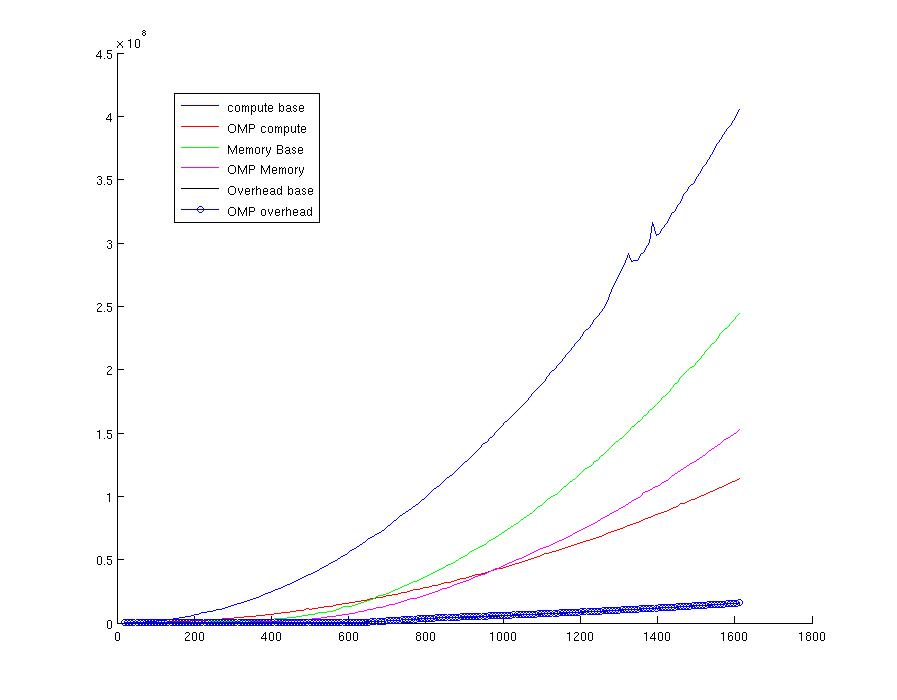
\includegraphics[scale=0.3]{part2}
\end{figure}

\section{Part Three -- Matrix Multiply}

	\subsection{Part A}
	
	\subsection{Part B}
	
	\subsection{Part C}
	
\section{Part Four -- Open MP with Real Programs}	
	
\end{document}	
